\setcounter{page}{3}

\chapter{Задание}

\textbf{Цель работы:} построение гистограммы и эмпирической функции распределения.

Содержание работы:
\begin{enumerate}
	\item Для выборки объема $n$ из генеральной совокупности $X$ реализовать в виде программы на ЭВМ: \begin{itemize}
		\item вычисление максимального значения $M_max$ и минимального значения $M_min$;
		\item размаха $R$ выборки;
		\item вычисление оценок $\hat{\mu}$ и $S^2$ математического ожидания $MX$ и дисперсии $DX$;
		\item группировку значений выборки в $m = [\log_2{n}] + 2$ интервала;
		\item построение на одной координатной плоскости гистограммы и графика функции плотности распределения вероятностей нормальной случайной величины с математическим ожиданием $\hat{\mu}$ и дисперсией $S^2$;
		\item построение на другой координатной плоскости графика эмпирической функции распределения и функции распределения нормальной случайной величины с математическим ожиданием $\hat{\mu}$ и дисперсией $S^2$.
	\end{itemize}
	\item Провести вычисления и построить графики для выборки из индивидуального варианта.
\end{enumerate} 

Данные для лабораторной работы по индивидуальному варианту:

\begin{lstlisting}[]
X = [1.52, 1.26, 2.17, 1.75, -0.19, 2.24, 2.76, 1.52, 1.89, 3.10, 2.61, 1.18, 1.83, 1.85, 3.39, 2.31, 2.99, 1.61, 2.57, 1.81, 1.73, 1.89, -0.00, 2.27, 1.61, 2.57, 2.54, 1.67, 1.49, 0.12, -0.04, 1.36, 2.04, 2.04, -0.05, 0.67, 1.32, 0.78, 0.89, 2.73, 1.51, 1.48, 1.67, 2.18, 1.70, 4.20, 1.81, 2.66, 1.72, 0.77, 3.16, 1.86, 3.66, 4.30, 0.98, 3.00, 0.99, 1.72, 2.71, 2.47, 2.56, 1.99, 0.23, 0.66, 2.47, 2.71, 2.28, 2.59, 3.30, 2.08, 0.90, 0.49, 2.38, 0.71, 0.10, 1.50, 0.21, 0.44, 3.94, 1.50, 1.70, -0.73, 1.76, 2.71, 1.95, -0.71, 1.32, 3.95, 2.64, -0.04, 3.24, 1.67, 2.31, 0.18, 0.79, 3.26, 3.44, 2.64, 0.89, 2.47, 4.02, 2.12, 0.61, 2.59, 1.44, 1.82, 2.94, 3.03, 1.97, 2.30, 0.80, 0.52, 1.21, 2.13, 2.82, 1.56, 2.84, 3.54, 0.86, 0.42];
\end{lstlisting}

\chapter{Теоретическая часть}

\section{Формулы для вычисления величин}

Пусть $X$~---~случайная величина (СВ). Генеральной совокупностью называется множество всех возможных значений СВ $X$. 

Случайной выборкой из генеральной совокупности $X$ называется случайный вектор $\overrightarrow{X} = (X_1, X_2, ..., X_n)$, где $X_i$, $i = \overline{1, n}$~---~независимы в совокупности и имеют одинаковое с $X$ распределение. $n$ называют объемом случайной выборки.

Выборкой объема $n$ из генеральной совокупности $X$ называется любая реализация $\overline{x}$ случайной выборки $\overrightarrow{X}$ объёма $n$ из этой генеральной совокупности.

Пусть $\vec x=(x_1, ..., x_n)$~---~выборка из генеральной совокупности $X$.

Тогда:

\begin{enumerate}
 \item Максимальное $M_{max}$ и минимальное $M_{min}$ значение выборки: $M_{max} = max(x_1, .., x_n)$, $M_{min} = min(x_1, .., x_n)$;
 \item Размах R выборки: $R = M_{max} - M_{min}$;
 \item Оценки $\hat\mu$ и $S^2$ математического ожидания $MX$ и дисперсии $DX$:
  \begin{itemize}
   \item Выборочное среднее: $\hat\mu(\vec{x}) = \overline x = \frac{1}{n} \cdot \sum\limits_{i=1}^{n} x_i$;
   \item Исправленная выборочная дисперсия: $S^2(\vec{x}) = \frac{1}{n - 1} \cdot \sum\limits_{i=1}^{n} (x_i - \overline x)^2$.
  \end{itemize}
\end{enumerate}

\section{Определение эмпирической плотности и гистограммы}



Пусть $\vec x$~---~выборка из генеральной совокупности $X$. Расположим значения $x_1, x_2, ..., x_n$ в порядке неубывания: $x_{(1)} \leq x_{(2)} \leq ... \leq x_{(n)}$. Последовательность $x_{(1)}, x_{(2)}, ..., x_{(n)}$, удовлетворяющую правилу $x_{(1)} \leq x_{(2)} \leq ... \leq x_{(n)}$, называют вариационным рядом выборки $\vec x$. При этом $x_{(i)}$~---~$i$-ый член вариационного ряда.

Если объем $n$ выборки $\vec x$ велик, то значения $x_i$ группируют в интервальный статистический ряд. Для этого отрезок $J = [x_{(1)}, x_{(n)}]$ делят на $m$ равновеликих частей:

\begin{equation*}
 J_i = [x_{(1)} + (i - 1) \cdot \Delta, x_{(1)} + i \cdot \Delta),\quad i = \overline{1, m - 1}.
\end{equation*}

\begin{equation*}
 J_{m} = [x_{(1)} + (m - 1) \cdot \Delta, x_{(1)} + m \cdot \Delta].
\end{equation*}

\begin{equation*}
 \Delta = \frac{x_{(n)} - x_{(1)}}{m}.
\end{equation*}

\noindent Чаще выборку разбивают на $m=[\log_2n]+2$ интервалов, где $n$ -- размер выборки.

Интервальным статистическим рядом называется таблица вида:

\begin{table}[h!]
 \centering
 \begin{tabular}{|c|c|c|c|c|}
  \hline
  $J_1$ & ... & $J_i$ & ... & $J_m$ \\
  \hline
  $n_1$ & ... & $n_i$ & ... & $n_m$ \\
  \hline
 \end{tabular}
\end{table}

где $n_i$ -- количество элементов выборки $\vec x$, попавших в $J_i$, $\overline{1, m}$.

Эмпирической функцией плотности, отвечающей выборке $\vec x$, называется функция
\begin{equation}
 \hat f_n(x) =
 \begin{cases}
 \frac{n_i}{n \Delta}, x \in J_i, i = \overline{1; m}, \\
 0, \text{иначе}, \\
 \end{cases}
\end{equation}

\noindent где $n_i$ -- количество элементов выборки, входящих в полуинтервал.

\textbf{Гистограмма} -- это график функции $\hat f_n(x)$. 

\section{Эмпирическая функция распределения}

Пусть $\vec x = (x_1, ..., x_n)$ -- выборка из генеральной совокупности $X$. Обозначим $n(x, \vec x)$ -- число элементов $\vec x$, которые приняли значение меньше $x$.

~\

Эмпирической функцией распределения, отвечающей выборке $\vec{x}$, называют функцию $\hat{F}_n: \mathbb{R} \to \mathbb{R}$, определенную правилом: 

\begin{equation*}
 \hat{F}_n(x) = \frac{n(x, \vec x)}{n}, x \in \mathbb{R},
\end{equation*}

\noindent где $n(x, \vec x)$~---~количество элементов выборки $\vec x$, которые имеют значения, меньше $x$.

\section{Функция плотности и функция распределения нормальной случайной величины}

Говорят, что случайная величина $X$ распределена по нормальному закону с параметрами $m$ и $\sigma^2$, если функция плотности распределения вероятностей $X$ имеет вид:

\begin{equation*}
 f(x) = \frac{1}{\sigma \cdot \sqrt{(2 \cdot \pi)}} \cdot e^{-\frac{(x - m)^2}{2\sigma^2}}.
\end{equation*}

~\

Функция распределения случайной величины $X$, распределенной по нормальному закону, имеет вид:

\begin{equation*}
 F(x) = \frac{1}{\sigma \sqrt{2 \pi}} \cdot \int_{-\infty}^{x}e^{-\frac{(t - m)^2}{2\sigma^2}}\, dt.
\end{equation*}

\chapter{Практическая часть}

\section{Код программы}

\begin{lstlisting}
X = [1.52, 1.26, 2.17, 1.75, -0.19, 2.24, 2.76, 1.52, 1.89, 3.10, 2.61, 1.18, 1.83, 1.85, 3.39, 2.31, 2.99, 1.61, 2.57, 1.81, 1.73, 1.89, -0.00, 2.27, 1.61, 2.57, 2.54, 1.67, 1.49, 0.12, -0.04, 1.36, 2.04, 2.04, -0.05, 0.67, 1.32, 0.78, 0.89, 2.73, 1.51, 1.48, 1.67, 2.18, 1.70, 4.20, 1.81, 2.66, 1.72, 0.77, 3.16, 1.86, 3.66, 4.30, 0.98, 3.00, 0.99, 1.72, 2.71, 2.47, 2.56, 1.99, 0.23, 0.66, 2.47, 2.71, 2.28, 2.59, 3.30, 2.08, 0.90, 0.49, 2.38, 0.71, 0.10, 1.50, 0.21, 0.44, 3.94, 1.50, 1.70, -0.73, 1.76, 2.71, 1.95, -0.71, 1.32, 3.95, 2.64, -0.04, 3.24, 1.67, 2.31, 0.18, 0.79, 3.26, 3.44, 2.64, 0.89, 2.47, 4.02, 2.12, 0.61, 2.59, 1.44, 1.82, 2.94, 3.03, 1.97, 2.30, 0.80, 0.52, 1.21, 2.13, 2.82, 1.56, 2.84, 3.54, 0.86, 0.42];

M_max = max(X)
M_min = min(X)

R = M_max - M_min

n = length(X);

mu = sum(X) / n
s2 = sum((X - mu) .^ 2) / (n - 1)

m = round(log2(n)) + 2;

[counts, edges] = histcounts(X, m, 'BinLimits', [M_min, M_max])

delta = R / m;
step = delta / 10;
Xs = M_min:step:M_max;
Ys = normpdf(Xs, mu, sqrt(s2));

hold on;
h = histogram();
h.BinEdges = edges;
h.BinCounts = counts / (n * delta);

plot(Xs, Ys, "red");

figure;
hold on;

[Ye, Xe] = ecdf(X);
plot(Xe, Ye, "blue");

Xs1 = M_min:step:M_max;
Ys1 = normcdf(Xs1, mu, s2);
plot(Xs1, Ys1, "red");
\end{lstlisting}

\section{Результат работы программы}

\subsection{Числовые характеристики}
\begin{equation*}
 M_{\min} = -0.73, \quad M_{\max} = 4.3, \quad R = 5.03, \quad m = 9, \quad \hat\mu(\vec x) = 1.836, \quad S^2(\vec x) = 1.153 \\
\end{equation*}

\newpage

\subsection{Графики}

\begin{figure}[!h]
 \center{\includegraphics[width=0.7\textwidth]{images/1.png}}
 \caption{Гистограмма и график функции плотности распределения вероятностей нормальной случайной величины с математическим ожиданием $\hat\mu$ и дисперсией $S^2$}
\end{figure}

\begin{figure}[!h]
 \center{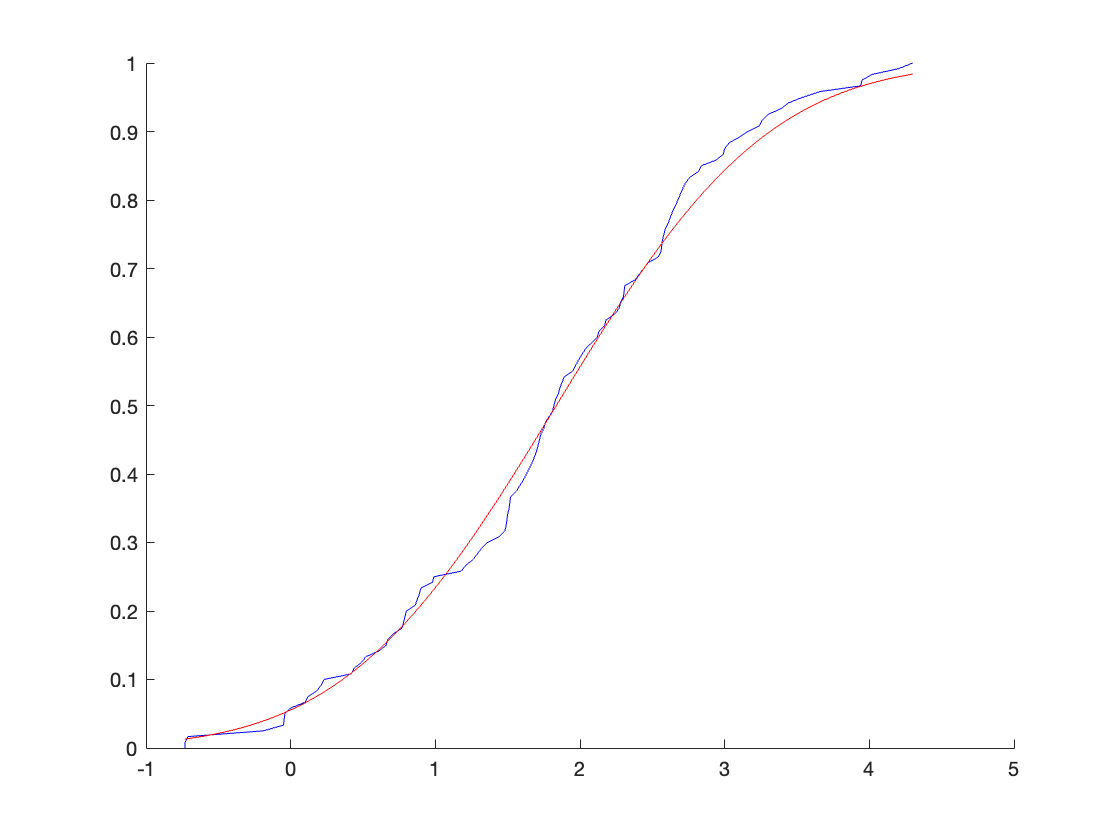
\includegraphics[width=0.7\textwidth]{images/2.png}}
 \caption{График эмпирической функции распределения и функции распределения нормальной случайной величины с математическим ожиданием $\hat\mu$ и дисперсией $S^2$}
\end{figure}



\newpage